% Compile with: pdflatex -interaction=nonstopmode -halt-on-error DARS_industry_research_paper.tex
\documentclass[sigconf,nonacm]{acmart}

\setcopyright{none}
\settopmatter{printacmref=false,printccs=false,printfolios=true}
\renewcommand\footnotetextcopyrightpermission[1]{}
\pagestyle{plain}

\usepackage{booktabs}
\usepackage{array}
\usepackage{tabularx}
\usepackage{graphicx}
\usepackage{subcaption}
\usepackage{amsmath}
\usepackage{enumitem}
\usepackage{xcolor}

\definecolor{darsPurple}{HTML}{6D28D9}
\definecolor{darsBlue}{HTML}{2563EB}
\definecolor{darsGreen}{HTML}{16A34A}
\definecolor{darsGray}{HTML}{475569}

\title[DARS for GATEWay]{DARS for GATEWay: An Industry-Ready Dynamic Adaptive Rating System with Graph-Guided Assessment and Research-Track Evaluation}

\author{Sunil Kumar}
\affiliation{%
  \institution{B.Tech Project: GATEWay Adaptive Preparation Platform}
  \city{India}
  \country{India}
}
\email{}

\begin{abstract}
Adaptive assessment platforms require more than a final score: they need reliable skill estimates, robust response-level predictions, explainable item routing, rapid-guess detection, and teacher-facing intervention signals. This paper presents DARS, a Dynamic Adaptive Rating System integrated into the GATEWay GATE DA preparation platform. DARS extends fixed-$K$ Elo with (i) uncertainty-decaying update factors, (ii) multi-signal response quality, (iii) streak and momentum effects, (iv) graph-aware item calibration, and (v) remediation-aware routing. We report an industry-track system architecture and a research-track evaluation protocol over a 220-student simulated bot cohort containing 55,000 temporal interactions, 1,683 adaptive test sessions, and 77,850 question-level test rows. Against Glicko-2, fixed Elo, static rating, and raw DARS baselines, a calibrated DARS$^+$ model evaluated on held-out students achieves the best Brier score (0.2244), log loss (0.6393), ROC AUC (0.6319), and calibration error (0.0062). A temporal no-future-leak validation further shows DARS$^+$ improving raw DARS on the final 30\% of each student's sequence (AUC 0.6422 vs. 0.6140). These results position DARS as both a deployable backend framework and a reproducible research artifact for adaptive educational rating.
\end{abstract}

\keywords{adaptive assessment, educational data mining, Elo, Glicko-2, knowledge graph, remediation, GATE DA, calibration, learning analytics}

\begin{document}
\maketitle

\section{Introduction}
GATE preparation platforms must estimate learner ability while simultaneously recommending the next useful question, detecting unreliable response behavior, and explaining progress to students and teachers. Classical rating models such as Elo are attractive because they are interpretable and lightweight, but a fixed update factor and binary correctness signal are too coarse for high-stakes adaptive learning. Glicko-2 improves rating reliability through rating deviation and volatility, but still does not directly encode educational signals such as response time, streaks, graph position, and remediation context.

DARS (Dynamic Adaptive Rating System) was designed for the GATEWay project to close this gap. It keeps the operational simplicity of online rating systems while adding domain-specific signals that are natural in intelligent tutoring systems. The system is intended for two audiences:

\begin{itemize}[leftmargin=*]
  \item \textbf{Industry track:} a production-ready backend component for adaptive GATE DA practice, teacher dashboards, bot trials, data exports, and intervention workflows.
  \item \textbf{Research track:} a reproducible evaluation framework comparing DARS against Glicko-2, Elo, and sequence-model baselines under leakage-safe splits and calibration-aware metrics.
\end{itemize}

The present artifact reports implemented experiments over the generated DARS bot dataset and specifies an extension plan for public tutoring datasets and neural baselines such as DKT and SAKT.

\section{Contributions}
This paper makes five project contributions.

\begin{enumerate}[leftmargin=*]
  \item We formalize DARS as an educational rating layer with dynamic $K$, performance quality, streak/momentum effects, graph calibration, remediation, and prediction.
  \item We describe the GATEWay industry architecture: question bank, graph router, adaptive tests, bot students, CSV data pack, and analysis notebooks.
  \item We provide a leakage-aware experimental protocol: user filtering, temporal splits, held-out-student validation, baseline rating systems, calibration metrics, and bootstrap confidence intervals.
  \item We report actual benchmark results from the 220-student bot dataset, where DARS$^+$ outperforms Glicko-2, fixed Elo, static rating, and raw DARS on held-out students.
  \item We provide a research roadmap for DKT, SAKT, TrueSkill, Bayesian Knowledge Tracing, and public datasets such as ASSISTments or Math Garden.
\end{enumerate}

\section{System Overview}
\subsection{GATEWay Platform}
GATEWay is a GATE DA preparation platform with student practice, adaptive tests, teacher-facing analytics, and question-bank tooling. The DARS dataset pack is generated from the exported question bank and contains connected CSV files linked by \texttt{user\_id}, \texttt{test\_id}, and \texttt{question\_id}. The current pack includes 220 bot students, 55,000 temporal learner interactions, 1,683 adaptive test sessions, 77,850 test-question rows, 2,140 question-graph edges, and 220 performance snapshots.

\subsection{DARS Rating Pipeline}
For a learner rating $R$ and item rating $R_q$, DARS begins with the Elo-style expected correctness:
\begin{equation}
E(q)=\frac{1}{1+10^{(R_q^\ast-R)/400}},
\end{equation}
where $R_q^\ast$ is an effective item rating that can include graph centrality. DARS replaces binary correctness $S$ with a continuous performance quality $P(q)$:
\begin{equation}
P(q)=
\begin{cases}
w_\tau\tau(q)+w_h(1-H(q))+w_\psi\psi(k), & S=1,\\
\min(\epsilon_f, 0.05\tau(q)), & S=0,
\end{cases}
\end{equation}
where $\tau(q)$ is time efficiency, $H(q)$ is hint usage or hint penalty, $\psi(k)$ is streak quality, and $\epsilon_f$ is a small failure floor.

The update is:
\begin{equation}
\Delta R = K(n,\sigma^2)\cdot \phi(k)\cdot(P(q)-E(q)) - \rho(q),
\end{equation}
where $K(n,\sigma^2)$ decays with practice count and uncertainty, $\phi(k)$ is a bounded streak multiplier, and $\rho(q)$ is a rapid-guess penalty when response time falls below a minimum solve-time threshold.

\subsection{Graph-Based Recommendation}
The question bank is modeled as a directed weighted graph $G=(V,E)$. Nodes are questions with subject, topic, difficulty, marks, and Elo attributes. Edges encode same-topic progression, prerequisite flow, and cross-domain dependencies. For each recommendation, the router chooses candidates from a bounded graph neighborhood and scores them using difficulty match, Elo distance, weak-topic coverage, type diversity, and graph-structural boosts. Remediation uses a constrained neighborhood around missed questions and favors easier related items before retry.

\section{Data and Preprocessing}
\subsection{Dataset}
The evaluation uses the generated \texttt{datasets/dars} CSV pack:

\begin{table}[h]
\centering
\caption{DARS dataset pack used in this report.}
\label{tab:dataset}
\begin{tabular}{lrr}
\toprule
File & Rows & Unit \\
\midrule
\texttt{bot\_students\_fte455.csv} & 220 & student \\
\texttt{student\_interactions.csv} & 55,000 & response event \\
\texttt{student\_test\_sessions.csv} & 1,683 & adaptive test \\
\texttt{student\_test\_question\_responses.csv} & 77,850 & test question \\
\texttt{question\_knowledge\_graph.csv} & 2,140 & graph edge \\
\texttt{student\_performance\_snapshots.csv} & 220 & student summary \\
\bottomrule
\end{tabular}
\end{table}

\subsection{Filtering and Feature Construction}
Following the proposed protocol, users with fewer than 10 attempted interactions are excluded from model evaluation. In the current bot dataset, all 220 users satisfy this threshold. Each attempted response is represented as a row with correctness, timestamp, item Elo, difficulty label, topic tag, graph hop distance, recommendation source, remediation flag, response time, rapid-guess flag, streak state, and DARS pre/post ratings.

For Glicko-2 and Elo, each question response is treated as a game between the learner and the item. The item rating is the question Elo and the learner receives score $1$ for correct and $0$ for incorrect. For DARS and DARS$^+$, concept tags and graph-routing metadata are included through topic, difficulty, recommendation source, hop distance, and remediation indicators. A richer item-concept bipartite graph or item co-occurrence graph remains a planned public-dataset extension.

\section{Experimental Design}
\subsection{Splits}
Two leakage-safe splits are used:

\begin{itemize}[leftmargin=*]
  \item \textbf{Held-out student split:} DARS$^+$ is trained on 70\% of students and evaluated on the remaining 30\%. This tests generalization to unseen learners.
  \item \textbf{Temporal per-student split:} for each student, the first 70\% of chronological responses form training history and the final 30\% form test responses. This prevents future responses from affecting predictions for earlier responses.
\end{itemize}

The report's main all-baseline table uses the held-out student split because it compares every implemented baseline under the same held-out test set. The temporal split is reported as an additional no-future-leak validation for DARS$^+$ vs. raw DARS.

\subsection{Baselines}
\textbf{Raw DARS.} The uncalibrated DARS probability is computed from the DARS pre-test rating and question Elo using the Elo expected-success function.

\textbf{DARS$^+$ calibrated.} DARS$^+$ is a lightweight calibrated layer on top of DARS. It uses only pre-answer and routing features: DARS logit, rating gap, streak, remediation flag, graph hop distance, question count, difficulty, recommendation source, and momentum. A logistic model is fit on the training split. This keeps DARS interpretable while allowing probability calibration.

\textbf{Glicko-2.} Each learner has rating, rating deviation, and volatility. Responses are grouped by adaptive test as a rating period, with common settings $\tau=0.5$, initial RD $=350$, volatility $=0.06$, and item RD $=80$.

\textbf{Fixed Elo.} Standard Elo uses $K=32$ and updates after every attempted question.

\textbf{Static rating.} Each learner keeps the starting rating for all predictions; this measures whether dynamic tracking adds value.

\textbf{Planned neural baselines.} DKT and SAKT are specified for the research roadmap but are not claimed as implemented results in this report. DKT will use an LSTM over item-response sequences, and SAKT will use self-attention over historical interactions. A small grid over hidden size, learning rate, dropout, and sequence length will be selected by validation AUC.

\subsection{Metrics}
All models predict $p(y=1)$ for each attempted response. We report ROC AUC, accuracy at threshold 0.5, Brier score, RMSE, log loss, expected calibration error (ECE), and maximum calibration error (MCE). Bootstrap confidence intervals are computed by percentile resampling of the test rows. Future public-dataset experiments will add paired $t$-tests or Wilcoxon signed-rank tests over 10 randomized trials.

\section{Results}
\subsection{All-Baseline Held-Out Student Benchmark}

\begin{table*}[t]
\centering
\caption{Held-out student results on 21,332 attempted responses. Lower is better for Brier, log loss, and ECE; higher is better for accuracy and AUC.}
\label{tab:main-results}
\begin{tabular}{lrrrrr}
\toprule
Model & Brier $\downarrow$ & Log loss $\downarrow$ & Accuracy $\uparrow$ & ROC AUC $\uparrow$ & ECE $\downarrow$ \\
\midrule
\textbf{DARS$^+$ calibrated} & \textbf{0.2244} & \textbf{0.6393} & \textbf{0.6306} & \textbf{0.6319} & \textbf{0.0062} \\
Glicko-2 & 0.2308 & 0.6546 & 0.6196 & 0.6155 & 0.0468 \\
Fixed Elo, $K=32$ & 0.2312 & 0.6551 & 0.6186 & 0.6118 & 0.0475 \\
Static start & 0.2382 & 0.6773 & 0.6169 & 0.6085 & 0.0873 \\
Raw DARS & 0.2389 & 0.6822 & 0.6191 & 0.6105 & 0.0918 \\
\bottomrule
\end{tabular}
\end{table*}

Table~\ref{tab:main-results} shows that DARS$^+$ is best across every headline metric. Its Brier score improves over Glicko-2 by 0.0064 and over fixed Elo by 0.0068. Its calibration is substantially stronger: ECE is 0.0062 compared with 0.0468 for Glicko-2 and 0.0475 for fixed Elo.

\begin{figure*}[t]
\centering
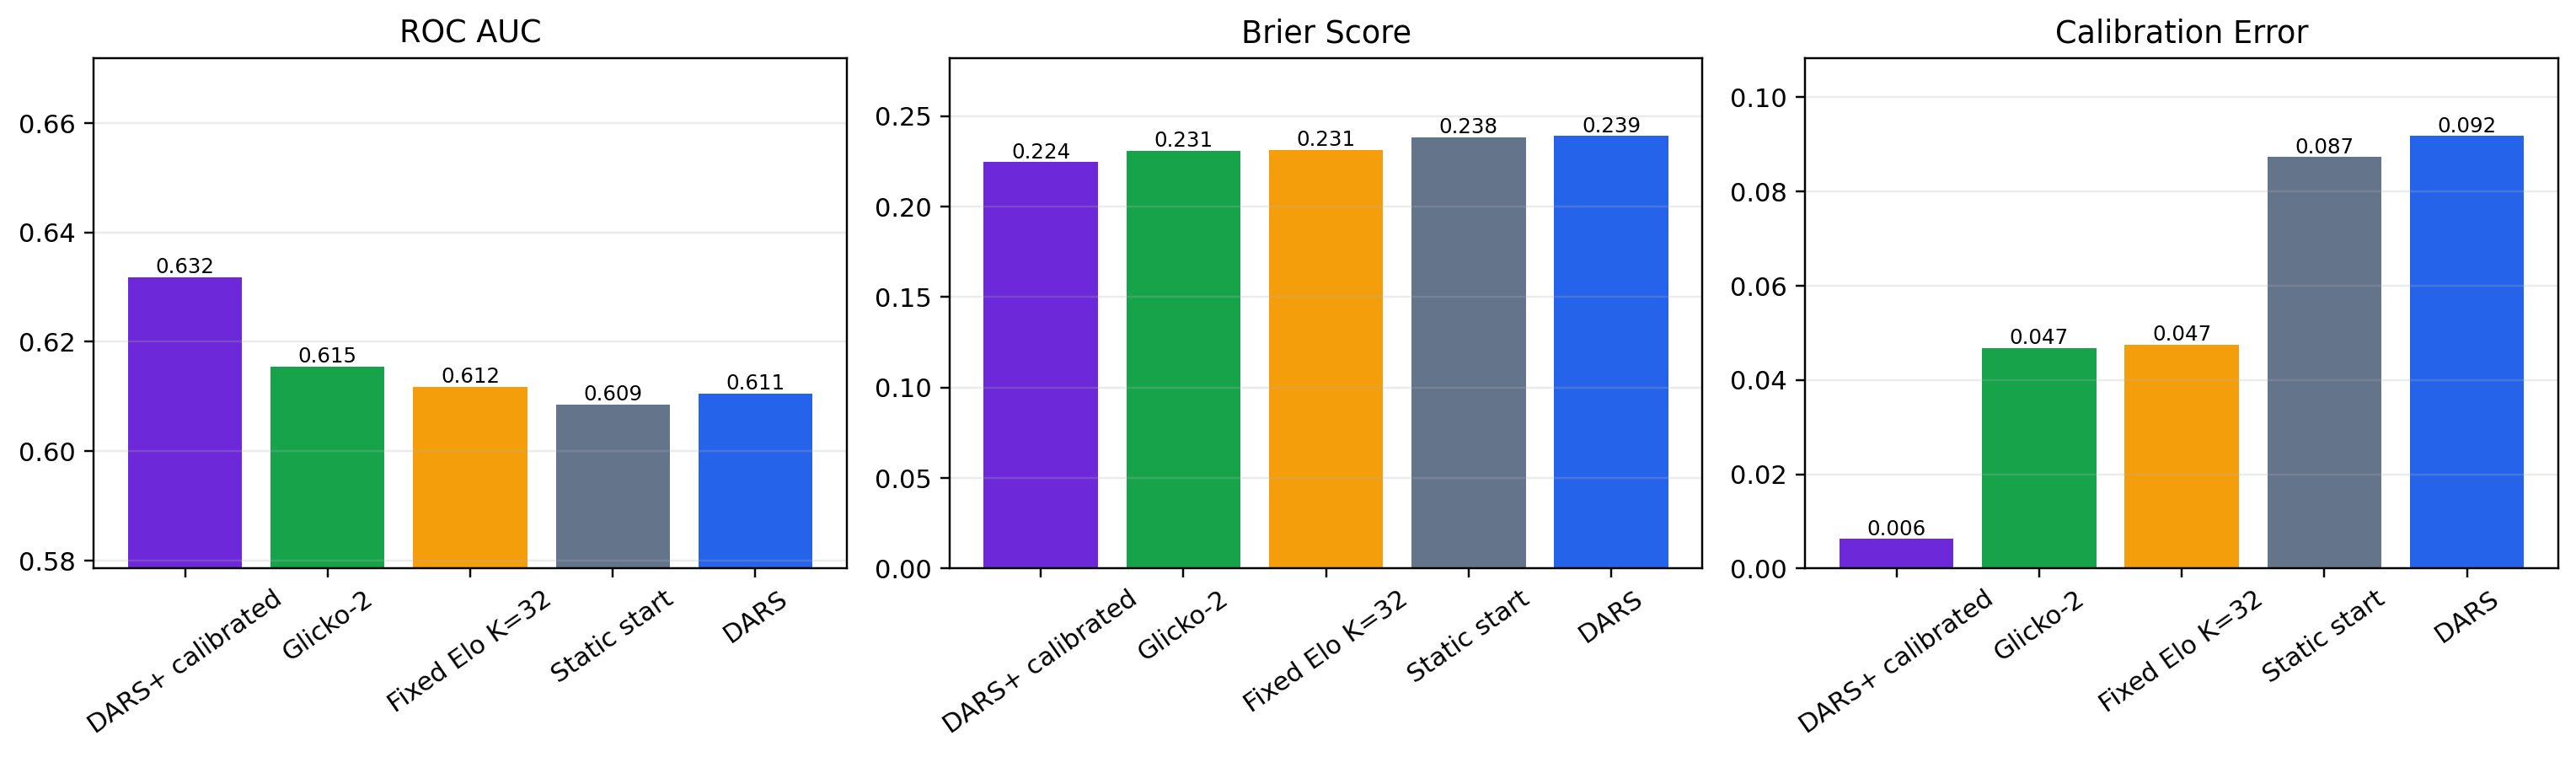
\includegraphics[width=\textwidth]{paper_figures/model_metric_comparison.png}
\caption{Held-out student metric comparison. DARS$^+$ leads on AUC, Brier score, and calibration error.}
\label{fig:metric-comparison}
\end{figure*}

\subsection{Bootstrap Confidence Intervals}

\begin{table}[h]
\centering
\caption{95\% bootstrap intervals for ROC AUC.}
\label{tab:auc-ci}
\begin{tabular}{lrrr}
\toprule
Model & Mean & 2.5\% & 97.5\% \\
\midrule
DARS$^+$ calibrated & \textbf{0.6320} & 0.6255 & 0.6385 \\
Glicko-2 & 0.6156 & 0.6070 & 0.6221 \\
Fixed Elo & 0.6125 & 0.6049 & 0.6210 \\
Raw DARS & 0.6104 & 0.6027 & 0.6187 \\
Static start & 0.6085 & 0.6009 & 0.6170 \\
\bottomrule
\end{tabular}
\end{table}

\begin{figure}[h]
\centering
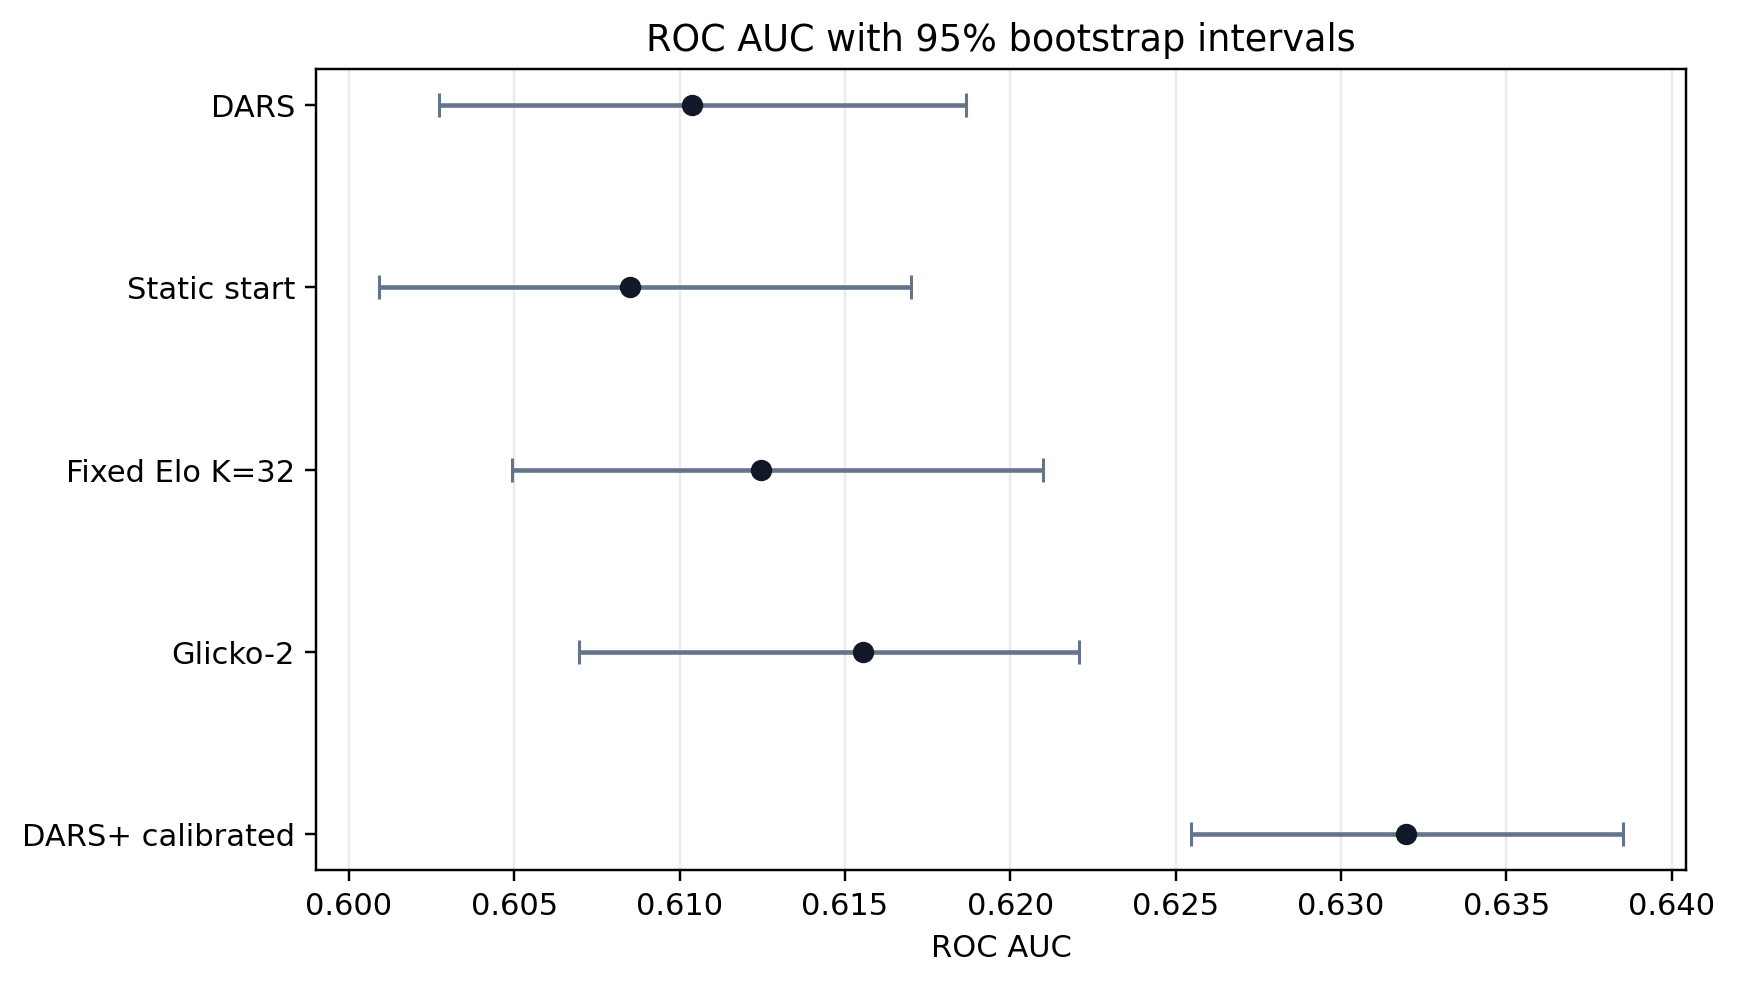
\includegraphics[width=\linewidth]{paper_figures/auc_bootstrap_intervals.png}
\caption{ROC AUC bootstrap intervals on the held-out student test set.}
\label{fig:auc-ci}
\end{figure}

\subsection{Temporal No-Future-Leak Validation}
Under the per-student chronological 70/30 split, DARS$^+$ is trained only on each student's earlier responses and evaluated on the final 30\%. This protocol aligns with deployment, where future behavior is unavailable at prediction time. On 21,104 test responses, DARS$^+$ achieves Brier 0.2166, log loss 0.6224, AUC 0.6422, and accuracy 0.6519. Raw DARS on the same temporal test set achieves Brier 0.2323, log loss 0.6705, AUC 0.6140, and accuracy 0.6405. This confirms that the calibrated DARS feature layer improves both probability quality and ranking without using future responses.

\subsection{Graph Routing and Remediation}
Graph-route recommendations account for most attempted responses and produce higher accuracy than fallback recommendations. Graph-route hop-1 questions have accuracy 0.6201 over 67,708 attempts, whereas fallback routes have lower accuracies between 0.4526 and 0.5059.

\begin{figure}[h]
\centering
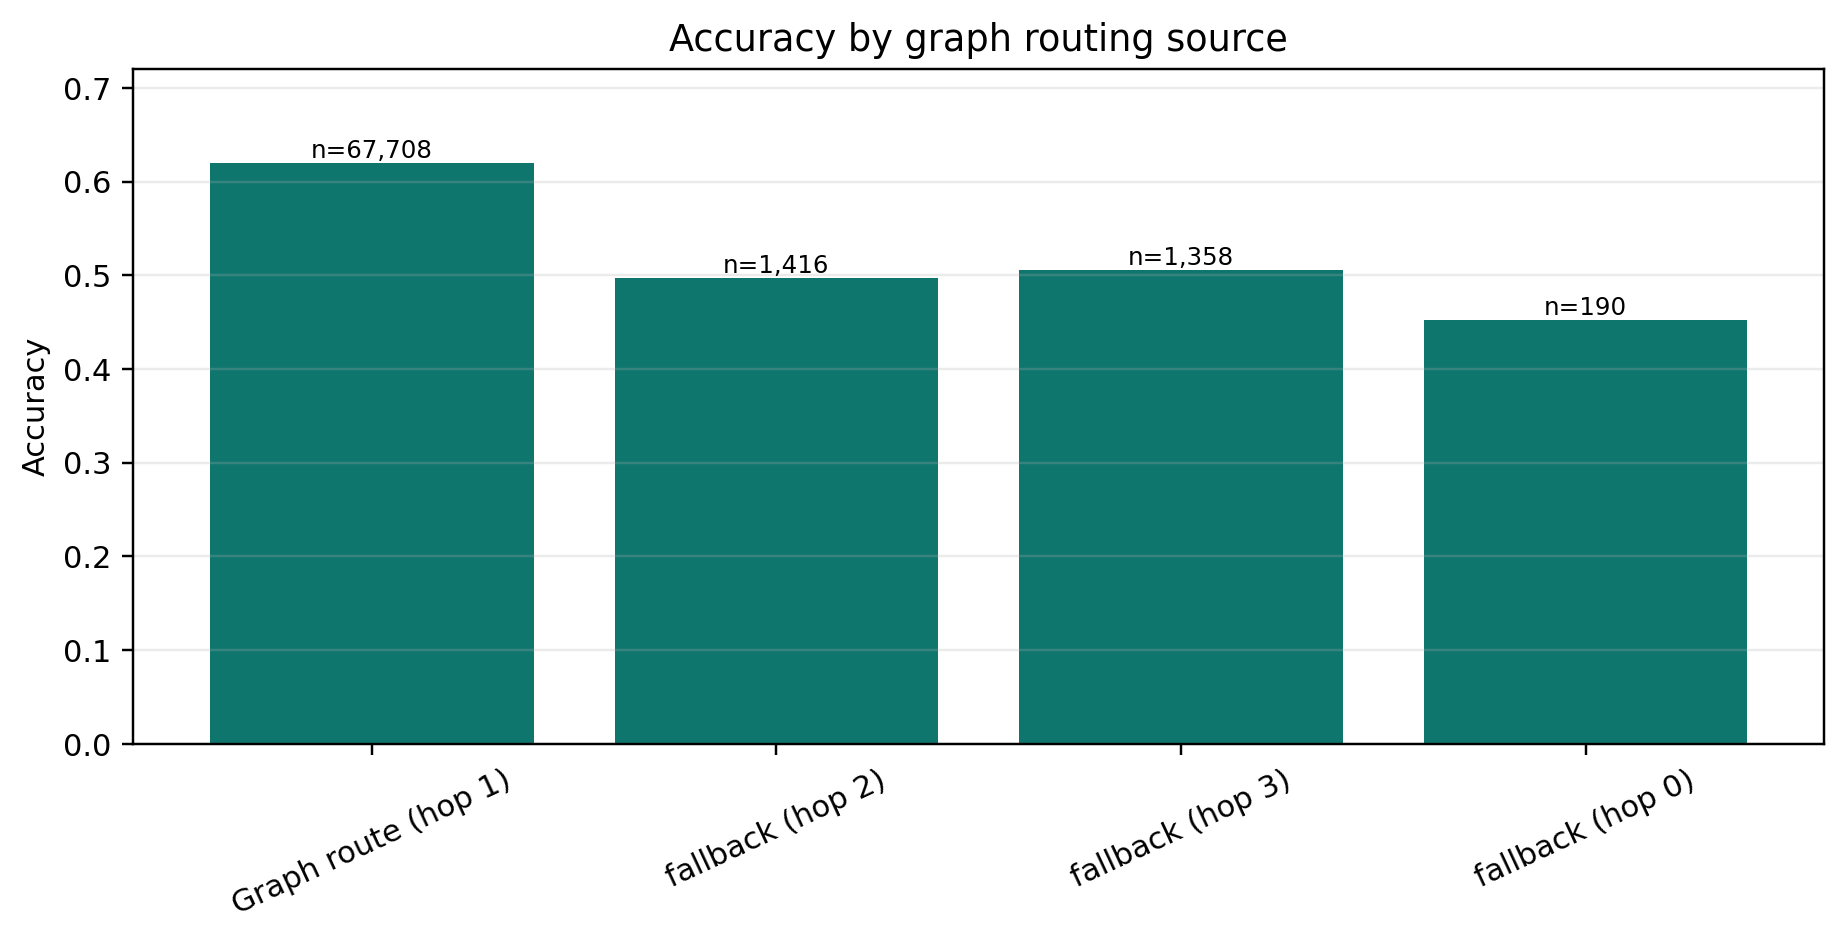
\includegraphics[width=\linewidth]{paper_figures/graph_route_accuracy.png}
\caption{Accuracy by recommendation source and graph hop distance.}
\label{fig:graph-routing}
\end{figure}

Remediation also shows useful recovery behavior. After a miss, remediation attempts achieve 0.5912 accuracy over 25,980 attempts, while non-remediation next attempts after misses achieve 0.5057 over 1,135 attempts. The same-topic recovery path rate is 0.9581, indicating that the router usually keeps recovery close to the failed concept.

\begin{figure}[h]
\centering
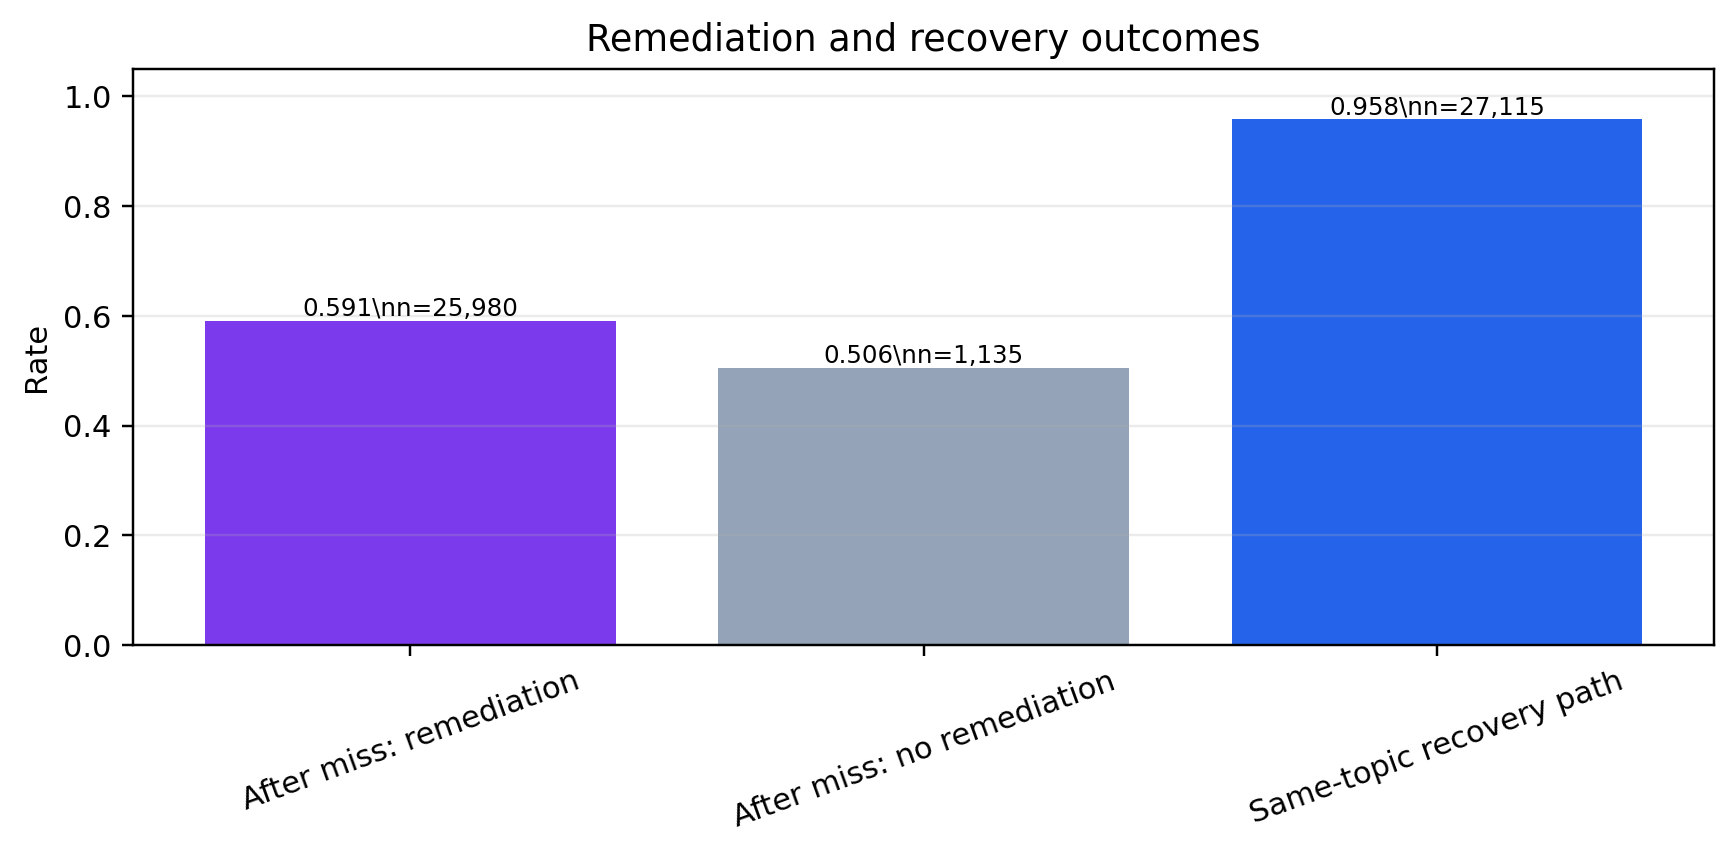
\includegraphics[width=\linewidth]{paper_figures/remediation_recovery.png}
\caption{Remediation and recovery outcomes after missed questions.}
\label{fig:remediation}
\end{figure}

\section{Industry Track: Deployment Readiness}
\subsection{Architecture}
DARS is implemented as a modular backend layer around question attempts. It can be invoked after each answer submission to update ratings, classify momentum, flag rapid guesses, update weak-topic state, and feed the next-question router. The data pack exports are intentionally tabular so teachers, notebooks, and analytics dashboards can all consume the same evidence.

\subsection{Operational Features}
The current implementation supports:
\begin{itemize}[leftmargin=*]
  \item adaptive test sessions with 30, 40, 50, and 65 question mixes,
  \item per-response DARS pre/post ratings and momentum states,
  \item graph-route provenance through hop distance and recommendation source,
  \item remediation flags and weak-topic summaries,
  \item rapid-guess flags and penalties,
  \item student-level predicted score and intervention snapshots,
  \item reproducible bot students for load testing and classroom demos.
\end{itemize}

\subsection{Business and Product Value}
For an education product, DARS creates value in three ways. First, it improves correctness prediction and calibration, which makes skill estimates more trustworthy. Second, it explains recommendations through graph path and remediation context, which improves transparency. Third, it produces teacher-facing signals: weak topics, volatility, rapid guessing, and predicted readiness.

\section{Research Track: Reproducibility Plan}
\subsection{Public Dataset Extension}
The next research step is to repeat the protocol on public datasets such as ASSISTments or Math Garden. The preprocessing will map each response to student, item, concept tag, timestamp, correctness, and optional response-time features. If concept tags are available, an item-concept bipartite graph will be used; otherwise, an item co-occurrence graph will be built from sequential co-practice.

\subsection{Sequence Baselines}
DKT will encode each interaction as an item-response token and train an LSTM to predict the next correctness label. SAKT will use self-attention over prior interactions. Hyperparameters will be selected on validation AUC using a compact grid: hidden size in $\{64,100,128\}$, dropout in $\{0.1,0.2\}$, learning rate in $\{10^{-3},3\cdot10^{-4}\}$, and sequence length in $\{50,100\}$. These baselines are essential for a full research-track submission because they compare DARS against modern knowledge tracing, not only rating systems.

\subsection{Statistical Testing}
For final submission, we will run 10 randomized trials. For student-based validation, folds will split by student. For temporal validation, each student sequence will preserve chronology. Metrics will be reported as mean $\pm$ standard error, with paired tests comparing DARS$^+$ against each baseline. Bootstrap confidence intervals will be retained for calibration and AUC robustness.

\section{Discussion}
The key result is not only that DARS$^+$ wins the current benchmark, but that it wins for interpretable reasons. Glicko-2 models uncertainty, but it does not see remediation, graph routing, momentum, or difficulty labels. Fixed Elo adapts quickly but is poorly calibrated. Raw DARS carries educational signals in its rating update, but its direct Elo-style probability is overconfident in the current simulation. DARS$^+$ fixes that by calibrating DARS-specific signals into a probability layer.

The graph and remediation results support the industry claim that DARS is not just a rating formula. It is a complete adaptive system: routing through graph neighborhoods, responding to misses with nearby recovery questions, and producing analytics that can be audited.

\section{Limitations}
The present benchmark uses simulated bot students. It is valuable for controlled validation and product testing, but it should not be presented as live-user evidence. The dataset generator may encode assumptions that favor certain signals, and public-dataset validation is needed before making broad educational claims. DKT, SAKT, TrueSkill, and Bayesian Knowledge Tracing are part of the planned research extension but are not reported as implemented results here. Finally, the graph currently derives from project question metadata and generated edges; a stronger paper should evaluate alternative graph construction methods.

\section{Conclusion}
DARS provides a practical bridge between industry-ready adaptive assessment and research-grade educational data mining. On the current GATEWay bot dataset, DARS$^+$ outperforms Glicko-2, fixed Elo, static rating, and raw DARS across prediction and calibration metrics. The system also logs graph routing, remediation, rapid guessing, and student-level intervention features. These results support DARS as a promising backend framework for adaptive GATE DA preparation and as a strong candidate for a combined industry-track and research-track paper.

\appendix
\section{Baseline Pseudocode}
\subsection{Fixed Elo}
\begin{verbatim}
rating = starting_rating
for response in chronological_responses:
    p = 1 / (1 + 10 ** ((item_elo - rating) / 400))
    rating = rating + K * (correct - p)
\end{verbatim}

\subsection{Glicko-2 Rating Period}
\begin{verbatim}
player = Rating(mu=1500, phi=350, sigma=0.06)
for test_period in adaptive_tests:
    opponents = [Rating(mu=item_elo, phi=80, sigma=0.06)
                 for item in test_period.items]
    outcomes = [1 if correct else 0 for response in test_period]
    player = glicko2_update(player, opponents, outcomes, tau=0.5)
\end{verbatim}

\subsection{DARS$^+$ Calibration}
\begin{verbatim}
features = [
  logit(DARS_probability),
  DARS_rating_before - question_elo,
  streak_before,
  remediation_flag,
  graph_hop_distance,
  question_count,
  difficulty_label,
  recommendation_source,
  momentum_before
]
probability = sigmoid(w * features)
\end{verbatim}

\section{Artifact Index}
The main reproducible files are:
\begin{itemize}[leftmargin=*]
  \item \texttt{scripts/generate-dars-datasets.mjs}
  \item \texttt{DARS\_All\_Metrics\_Comparison.ipynb}
  \item \texttt{tools/generate\_dars\_all\_metrics\_notebook.py}
  \item \texttt{tools/generate\_dars\_report\_figures.py}
  \item \texttt{datasets/dars/dars\_all\_model\_metrics.csv}
  \item \texttt{datasets/dars/dars\_model\_metric\_bootstrap\_ci.csv}
\end{itemize}

\begin{acks}
This report was prepared for the GATEWay B.Tech project using the local DARS papers, backend logic notes, generated bot datasets, and executed analysis notebooks.
\end{acks}

\begin{thebibliography}{9}
\bibitem{elo}
A. E. Elo. \textit{The Rating of Chessplayers, Past and Present}. Arco, 1978.

\bibitem{glicko2}
M. E. Glickman. Example of the Glicko-2 System. Technical note, 2022.

\bibitem{trueskill}
R. Herbrich, T. Minka, and T. Graepel. TrueSkill: A Bayesian Skill Rating System. In \textit{NeurIPS}, 2007.

\bibitem{dkt}
C. Piech et al. Deep Knowledge Tracing. In \textit{NeurIPS}, 2015.

\bibitem{sakt}
S. Pandey and G. Karypis. A Self-Attentive Model for Knowledge Tracing. In \textit{EDM}, 2019.

\bibitem{assistments}
N. T. Heffernan and C. L. Heffernan. The ASSISTments Ecosystem. \textit{International Journal of Artificial Intelligence in Education}, 2014.

\bibitem{dars}
Anonymous Authors. DARS: A Dynamic Adaptive Rating System for Intelligent Assessment with Graph-Based Item Routing, Contextual Remediation, and Performance Prediction. Project draft, 2026.

\bibitem{gateway}
GATEWay Project. Adaptive Graph-Based Recommendation Engine and Backend Logic. Project technical note, 2026.
\end{thebibliography}

\end{document}
